\section{L'analyseur de XML}

    \subsection{Les différentes classes}
    
    \begin{center}
    \begin{figure}[h]
        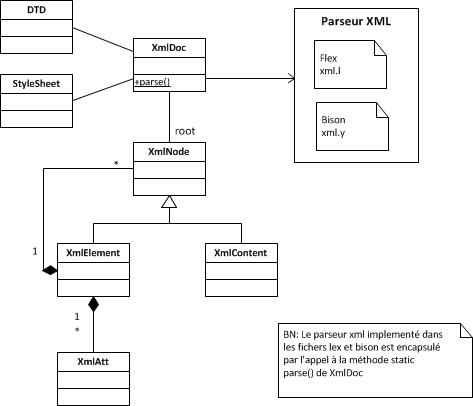
\includegraphics[width=15cm]{\PIXPATH/uml_xml}
        \caption{Diagramme UML simlpifié représentant les classes
                                                    de l'analyseur XML}
        \label{umlxml}
    \end{figure}
    \end{center}

    \subsection{Fonctionnement}

    Il est possible de~:

        \subsubsection{Parser un document XML et créer sa représentation 
                                                                en mémoire}

        En faisant appel à la méthode statique
        {\tt XmlDoc::parse( const \& nomFichier )},
        qui va se charger de lire le fichier, de l'analyser et de construire la
        structure du fichier en mémoire, comme indiqué sur le diagramme UML de
        la figure \ref{umlxml}. 

        \subsubsection{Afficher le document en mémoire}

        En faisant appel à la méthode {\tt XmlDoc::Display()}, on peut générer
        et afficher le contenu du fichier XML représenté en mémoire.

        \subsubsection{Valider le fichier XML}

        En faisant appel à {\tt XmlDoc::Validate( DTDDocument * dtd )}, on peut
        valider la conformité du document XML à la DTD {\tt dtd} passée en
        paramètre.

        Le mécanisme de validation est présenté en section \ref{valid}.
